In the proposed architecture, the \textit{Smart Gateway} is the central module of the system, connecting the \textit{Smart boxes} to the \acs{HIS}. It is responsible for the management of devices and their associations -- \textit{Smart box} to \textit{Biosticker} and \textit{Smart box} to user -- managing, maintaining and storing the data that is generated by these, as well as handling any communication to and from the \acs{HIS}. 


\paragraph{} Regarding the hardware platform used for the \textit{Smart Gateway}, in the context of the \acs{WoW} project, the Intel NUC NUC8i7BEH\footnote{\url{https://ark.intel.com/content/www/us/en/ark/products/126140/intel-nuc-kit-nuc8i7beh.html}} is used, as seen in Figure \ref{fig:gateway_image}. Table \ref{tab:NUCspecification} shows the hardware specification of the Intel NUC kit used.


\begin{figure}[H]
    \centering
    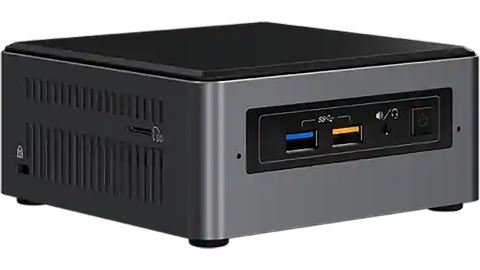
\includegraphics[width=0.4\linewidth]{images/gateway-image.png}
    \caption[Intel NUC NUC8i7BEH.]{Intel NUC NUC8i7BEH.}
    \label{fig:gateway_image}
\end{figure}

\begin{table}[H]
    \centering
    \caption{Intel NUC Kit NUC8i7BEH specification.}
    \label{tab:NUCspecification}
    \begin{tabular}{l|l}
    \hline
     \textbf{Memory}                     & 16 GB DDR4-2400MHz                                   \\ \hline
     \textbf{CPU}                        & Intel Core i7-8559U Processor (8M Cache, up to 4.50 GHz) \\ \hline
     \textbf{GPU}                         & Iris Plus Graphics 655                                     \\ \hline
     \textbf{Mass Storage}               & 1 TB SSD                                                      \\ \hline %32 GB 
     \textbf{Operating System}           & Ubuntu Server 20.04.2 LTS                                  \\ \hline
    \end{tabular}
\end{table}

\paragraph{} In the next sections, a service architecture for the \textit{Smart Gateway} is proposed in order to fulfill the aforementioned features.

% The \textit{Smart Gateway} maintains a list of all the \textit{Smart boxes} that are managed by the system, as well as every \textit{Biosticker} and every sensor in the \textit{Biosticker} (which are used to indicate respective biosignal to the \acs{HIS}). 


\section{Service Architecture}

As seen in Section \ref{sec:statement_of_contrib}, there are multiple key features that form the \textit{Smart Gateway}. The different \textit{Smart Gateway} components are:  

\begin{itemize}
    \item \textbf{Manage devices and device associations}: The \textit{Smart Gateway} maintains a list of all the \textit{Smart boxes} that are managed by the system, as well as every \textit{Biosticker} and every sensor in the \textit{Biosticker} (which are used to indicate the respective biosignal to the \acs{HIS}). The \textit{Smart Gateway} also tracks the sensor subscriptions per \textit{Smart box}.
    \item \textbf{Data anonymization}: Any private data (\textit{i.e.} information that can be used to identify a user) that is stored in the \textit{Smart Gateway} is anonymized in order to meet data protection regulations\footnote{Resolution of the Council of Ministers no. 41/2018, of 28 March, following the new General Data Protection Regulation (GDPR), approved by Regulation (EU) 2016/679:  \url{https://dre.pt/application/file/a/114936962\%20}}. 
    \item \textbf{Data pre-processing}: The \textit{Smart Gateway} processes the data as it is collected in order to clean the data before storing it indefinitely, and to detect critical conditions of the patients' state to prompt an immediate notification to the health professionals.
    \item \textbf{Real-time data acquisition}: The \textit{Smart Gateway} handles the secure communications with the \textit{Smart boxes}, acquiring the data in real-time.
    \item \textbf{Manage data collection}: After receiving and processing the data from the \textit{Smart boxes}, the \textit{Smart Gateway} stores indefinitely for long-term biomonitoring analytics.
    \item \textbf{\acs{HIS} \acs{FHIR} Integration}: The \textit{Smart Gateway} handles the communication with the \acs{HIS}. More specifically, it processes all \acs{FHIR} requests from the \acs{HIS}, and also transforms the acquired sensor data into \acs{FHIR} messages and communicates it to the \acs{HIS}. 
\end{itemize}

To implement these components,  the following service architecture within the \textit{Smart Gateway} is proposed, as illustrated in Figure \ref{fig:gateway_serviceoverview}. The correspondence between the services and the \textit{Smart Gateway} components is described in Table \ref{tab:gateway-service}.

\begin{figure}[H]
    \centering
    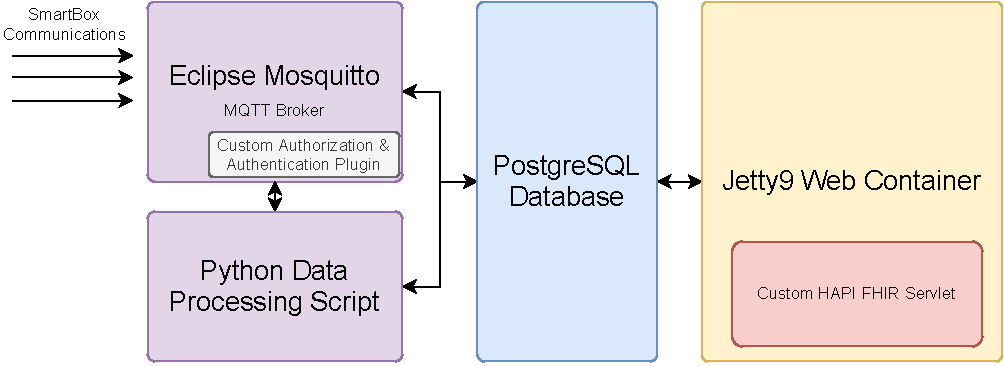
\includegraphics[width=0.93\linewidth]{images/service overview gateway.pdf}
    \caption[Service architecture implemented in the \textit{Smart Gateway}.]{Service architecture implemented in the \textit{Smart Gateway}. The diagram displays the different technologies used throughout the development.}
    \label{fig:gateway_serviceoverview}
\end{figure}
\begin{table}[H]
    \caption{Correspondence between the \textit{Smart Gateway} services and its functional components.}
    \label{tab:gateway-service}
    \resizebox{\textwidth}{!}{%
    \begin{tabular}{ccc}
    \hline
    \textbf{\textit{Smart Gateway} Component}          & \textbf{\textit{Smart Gateway} Service} & \textbf{Description}                                                                                                                                                             \\ \hline
    Real-time data acquisition             & MQTT Broker                   & \makecell[c]{Service that handles communication with \\the \textit{Smart boxes}, ensuring data\\  encryption, authorization, etc.}                                                           \\ \hline
    Data pre-processing                    & Data processing               & \makecell[c]{Data filtering and preliminary data \\ processing.}                                                                                                  \\ \hline
    \multirow{3}{*}{\makecell[c]{Manage data collection \\ Manage devices and device associations}}                & \multirow{3}{*}{Data storage} & \multirow{3}{*}{\makecell[c]{Management and storage system information,\\ such as the list of devices, permissions of each \\ device and collected sensor data.}} \\
     &                               &                                                                                                                                                                                  \\ & & \\ \hline
    Data anonymization                     & \multirow{2}{*}{FHIR Server}  & \multirow{2}{*}{\makecell[c]{Service that handles communications with\\ the  ``Interoperability'' layer  of \acs{HIS}.}}                                                         \\ 
    \acs{HIS} \acs{FHIR} Integration       &                               &              \\\hline                                                                                                                                                                   
    \end{tabular}
    }
\end{table}

\paragraph{} The services communicate with one another using UNIX Domain Sockets\footnote{\url{https://man7.org/linux/man-pages/man7/unix.7.html}}. This is an interprocess communication (\acs{IPC}) protocol that enables efficient communication between processes running on the same host operative system. This protocol is very efficient, compared for example to traditional network sockets \cite{Wright2007}, since all communication is handled entirely by the operative system kernel, instead of relying on the \acs{IP} protocol stack, minimizing communication overhead. 

The protocol can make use of the Linux file system for addressing the sockets, which means it is subject to Linux file system permissions. This allows applications to identify which process, or more accurately, the user running the process, who is attempting to establish a new connection to that application, providing a simple and secure authentication mechanism on the \acs{IPC}.

\section{Data Storage}

Data storage in the \textit{Smart Gateway} is one of the most important components of the device, as it holds the information used by all services in the \textit{Smart Gateway}. Given the importance of this component, it is crucial to use a solution which offers reliability above all, with proved performance for our use case.  

\paragraph{} As discussed in Section \ref{sec:iot-model-layer4}, No\acs{SQL} databases are appealing for \acs{IoT} applications, since these can handle unstructured or semi-structured data and generally perform better than traditional \acs{SQL} databases as the amount of data stored increases. However, these systems are not adequate for a relational data model, which is required to enforce consistent and logical representation of information. For this reason, a traditional \acf{RDBMS} has been deployed for data storage in the system.

\paragraph{} Out of the different \acs{RDBMS}s available in the market, PostgreSQL stands out due to its overall performance and scalability \cite{Asiminidis2018}. Additionally, it is one of the most popular \acs{RDBMS} \cite{dbengines}, meaning it also has significant community support. 

\paragraph{} With this in mind, PostgreSQL has been chosen as the data storage technology in the \textit{Smart Gateway}. PostgreSQL\footnote{\url{https://www.postgresql.org}} is an advanced, enterprise-class, and open-source \acs{RDBMS}. It has over 30 years of active development by the open source community, earning a strong reputation for its reliability, feature set and robustness.

\subsection{Database Schema}
Figure \ref{fig:wow-dbschema-full} contains the database model implemented in our PostgreSQL database. It describes all information that is contained in the \textit{Smart Gateway}, the relations within that data, organized according to how that information is used (\textit{i.e.} the service / functionality it is associated with). The data stored in the system can be categorized into 5 distinct groups:

\begin{enumerate}
    \item \textbf{System data} -- Information about the devices which are managed by the system: the \textit{Smart boxes}, the \textit{Biostickers} and the sensors in each \textit{Biostickers}. 
    \item \textbf{\acs{MQTT} related data} -- Information about the \acs{MQTT} clients and their permissions. 
    \begin{figure}[H]
        \centering
        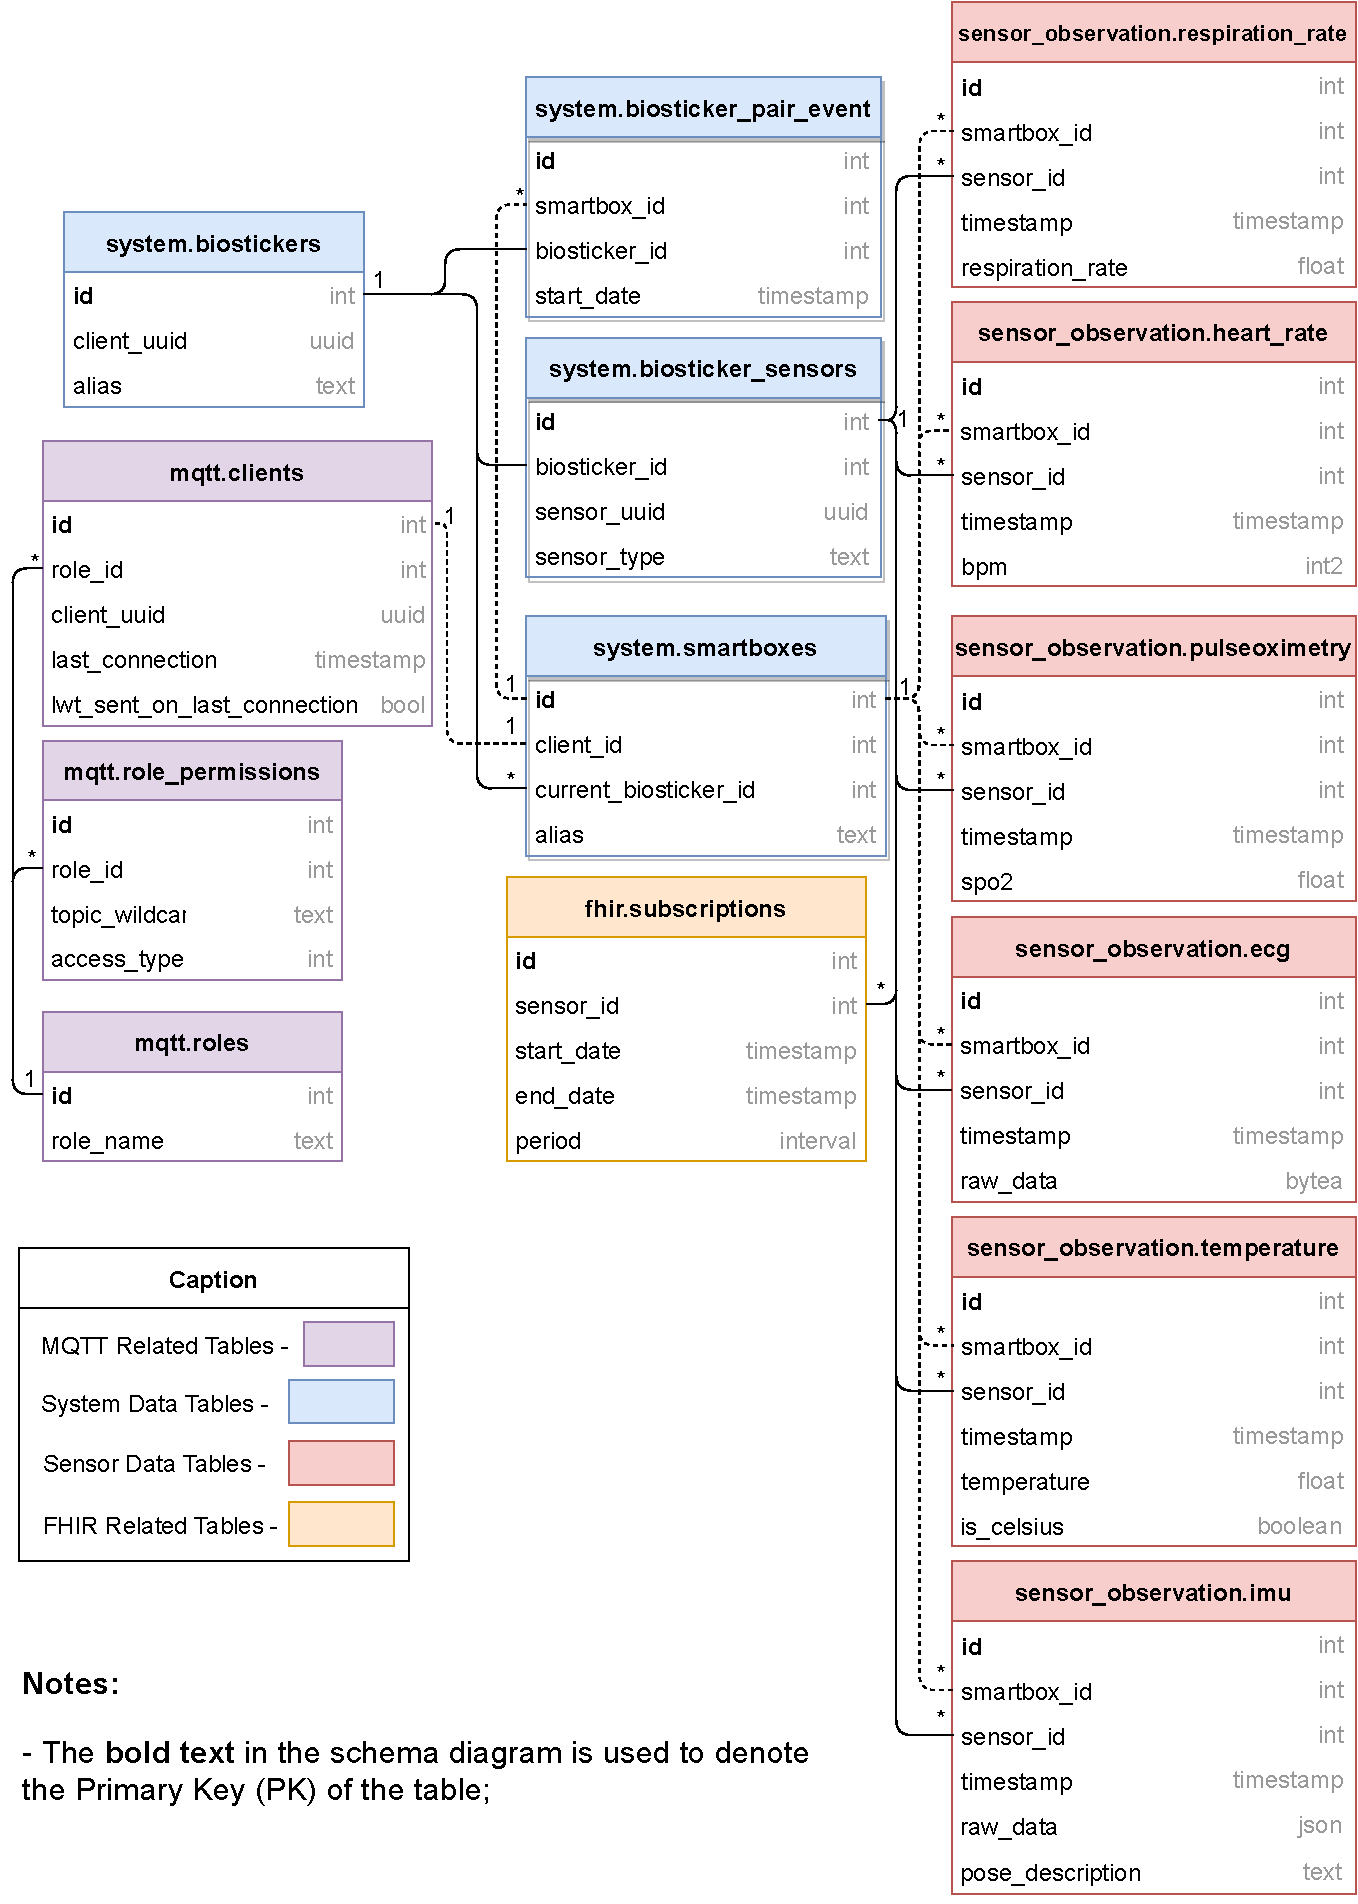
\includegraphics[width=0.9\linewidth]{images/database-schema-general.pdf}
        \caption[Database model implemented in the \textit{Smart Gateway}.]{Database model implemented in the \textit{Smart Gateway}. The bold text in the diagram is used to denote the Primary Key (PK) of each table. The relationships between entities are indicated with a line and using the symbols ``*'' for many and ``1'' for one.}
        \label{fig:wow-dbschema-full}
    \end{figure}
    \item \textbf{Sensor observation data} -- Biosignals measured and communicated by the \textit{Smart boxes}.
    \item \textbf{\acs{FHIR} data} -- Data related with \acs{FHIR} communications, such as the subscription requests from the \acs{HIS} to communicate the acquired sensor measurements.
    \item \textbf{Stored procedures} -- Custom subroutines that define the operations used by other services (\textit{e.g.} the \acs{MQTT} broker) to interact with the stored data (insertions, deletions, searches, etc.).
\end{enumerate}

%\clearpage 

In the next sections, the structure of the data within each of these groups is explored in greater detail.

\subsubsection{System data}
\paragraph{} Figure \ref{fig:wow-dbschema-system} describes the components or entities of the database model that depict system information. The data model is designed with flexibility in mind, allowing each \textit{Smart box} to be associated with any number of \textit{Biostickers}, and each \textit{Biosticker} to have any number of sensors associated to it. 

\paragraph{} Each sensor is uniquely identified by an \acs{UUID} when communicating the sensor measurement to the \acs{HIS}. As the names suggest, the ``system.biostickers'' table contains the list and details of all \textit{Biostickers}, ``system.smartboxes'' table contains the list and details of all \textit{Smart boxes}, ``system.biosticker\_sensors'' contains the list and details of all sensors of all \textit{Biostickers}. The ``system.biosticker\_pair\_event'' table is used to track the history of which \textit{Biostickers} were or are currently associated with a specific \textit{Smart box}.

\begin{figure}[H]
    \centering
    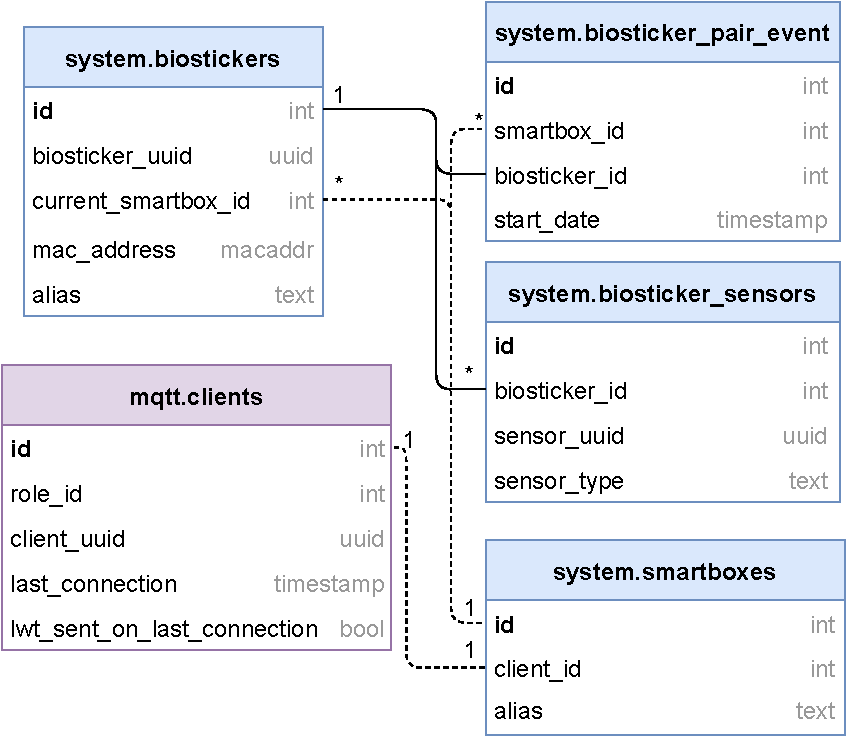
\includegraphics[width=0.55\linewidth]{images/database-schema-system.pdf}
    \caption{
    Components of the database model used to describe system information.}
    \label{fig:wow-dbschema-system}
\end{figure}

\subsubsection{MQTT related data}

\paragraph{} Figure \ref{fig:wow-dbschema-mqtt} describes the information relevant for \acs{MQTT} communications, mostly related with security. To ensure that each device only has access to allowed resources, the system implements a role-based access control (\acs{RBAC}) policy. 
In this type of access control, the system allows or revokes access to resources according to the role of the device, meaning that all devices with a given role share the same list of permissions. The permissions for the \acs{RBAC} policy contain 3 properties: the ID of the role it applies to, the topic name, and the level of access (PUBLISH, SUBSCRIBE and/or READ) to be granted (or revoked), as seen in Figure \ref{fig:wow-dbschema-mqtt}. READ access in this context is the ability to receive messages from the broker when subscribed to that topic. SUBSCRIBE access is the ability to issue a subscription request, and PUBLISH the ability to publish messages.

\paragraph{} In context of the \acs{WoW} project, the following roles are used:

\begin{itemize}
    \item \textit{Smart box} role: Indicates that the \acs{MQTT} client is a \textit{Smart box}.
    \item ``Pyservice'' role: Indicates that the \acs{MQTT} client is actually the data pre-processing service, also contained in the \textit{Smart Gateway}.
    \item Developer device role: Indicates that the \acs{MQTT} client is a developer device, used solely for debugging purposes.
\end{itemize}

\paragraph{} The ``mqtt.roles'' table contains the different \acs{RBAC} roles for the \acs{MQTT} communication and ``mqtt.role\_permissions'' table lists the permissions available to each role using \acs{MQTT} topic wildcards. The ``mqtt.client'' table lists the clients and their properties, such as their \acs{UUID}, the timestamp of their last connection, or a \textit{flag} to indicate if the communication failed during the last communication.

\begin{figure}[H]
    \centering
    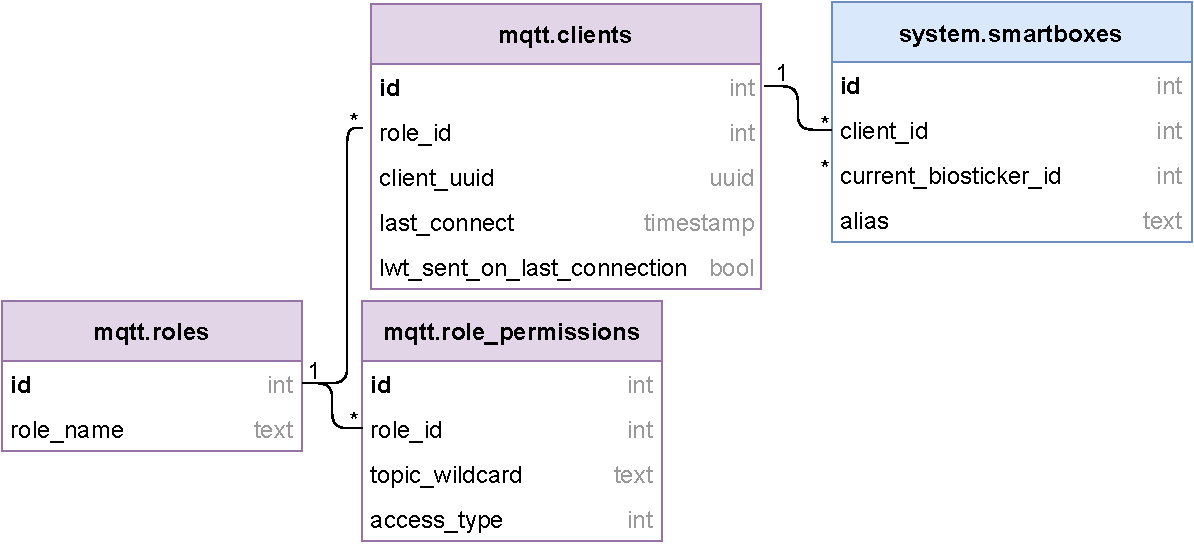
\includegraphics[width=0.75\linewidth]{images/database-schema-mqtt.pdf}
    \caption{Components of the database model used to describe \acs{MQTT} information. }
    \label{fig:wow-dbschema-mqtt}
\end{figure}


\subsubsection{Sensor observation data}

\paragraph{} Figure \ref{fig:wow-dbschema-sensors} describes the information of the sensor measurements collected over time. Each signal measurement is associated with the sensor that measured it and the \textit{Smart box} that is associated to that sensor, or more accurately, associated to the \textit{Biosticker}, at the moment of the observation.

\paragraph{} The database model has one table for each type of biosignal measured in the \acs{WoW} project (temperature, \acs{ECG}, etc.). The properties of the table are defined according to the structure of the data that is acquired by the \textit{Smart box}, which are detailed in Section \ref{sec:biosticker_data}. The ``pose\_description'' field in ``sensor\_observations.imu'' table is a text representation of the different body poses according to an international health standard\footnote{\url{https://loinc.org/8361-8/}}.

\begin{figure}[H]
    \centering
    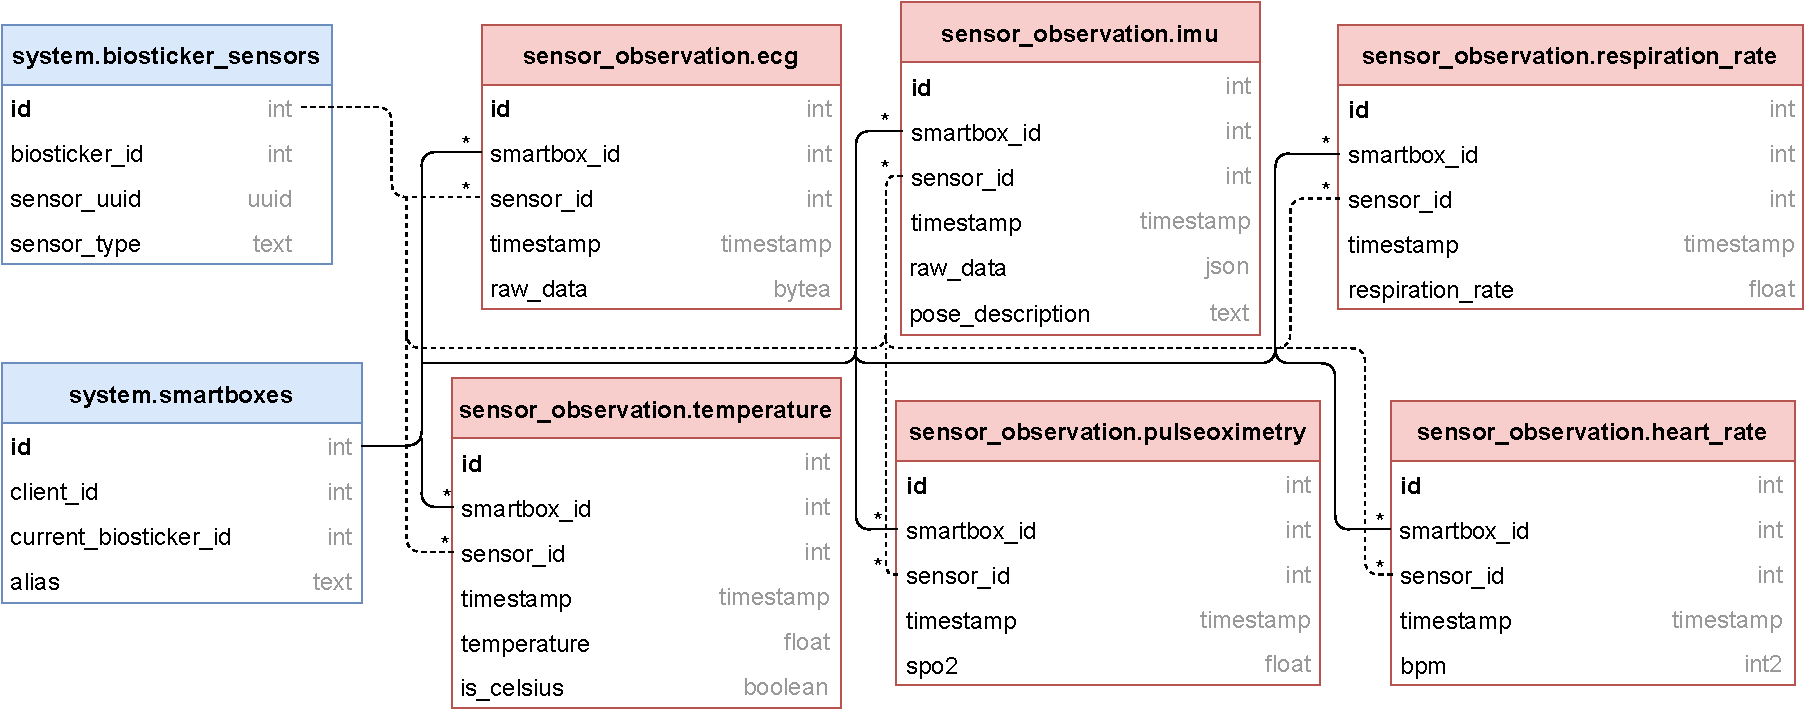
\includegraphics[width=\linewidth]{images/database-schema-sensordata.pdf}
    \caption{Components of the database model used to describe sensor measurements. }
    \label{fig:wow-dbschema-sensors}
\end{figure}



\subsubsection{\acs{FHIR} data}

Figure \ref{fig:wow-dbschema-fhir} describes the information associated with the \acs{FHIR} communications. Currently, the only information that is stored in the database is the list of subscription requests sent from the \acs{HIS}. The ``status'' field in the ``fhir.subscription'' table indicates the status of the subscription request (active, completed, revoked, etc.) and should be a text value that matches its equivalent in the \acs{FHIR} enumeration \cite{fhir}.

\begin{figure}[H]
    \centering
    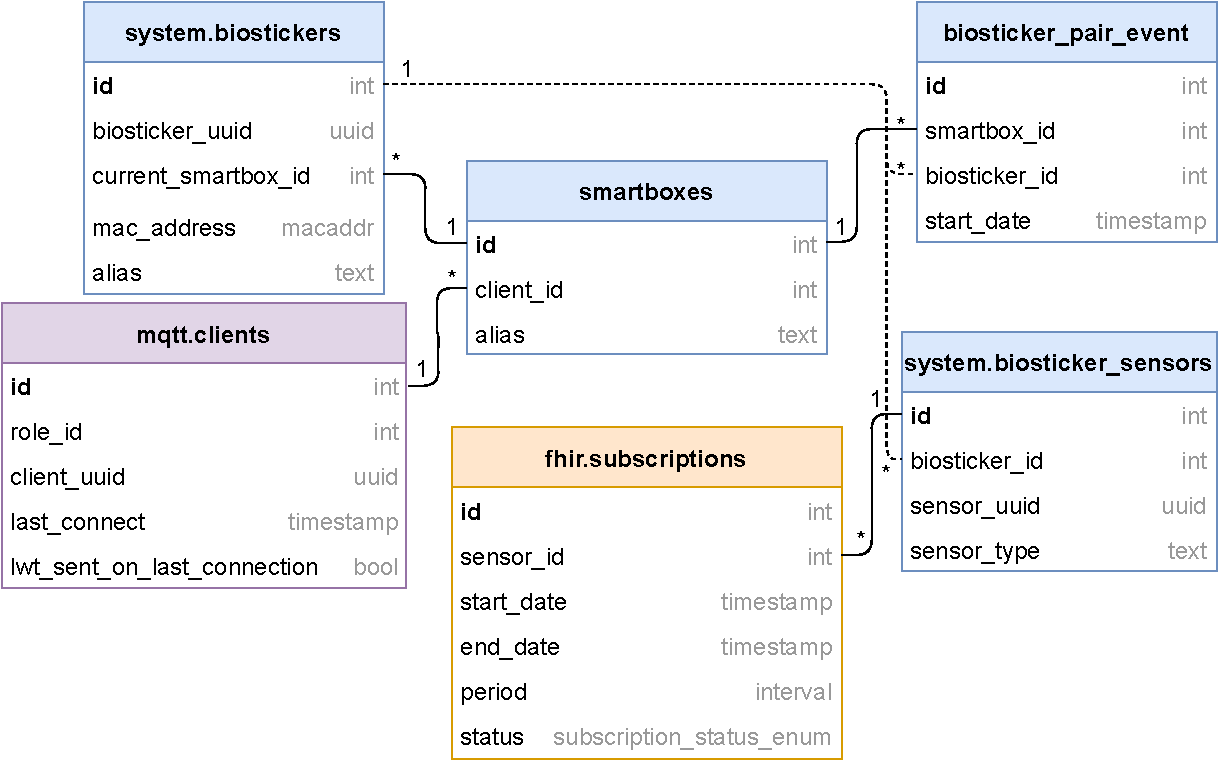
\includegraphics[width=0.66\linewidth]{images/database-schema-fhir.pdf}
    \caption{Components of the database model used to describe information used for \acs{FHIR}.}
    \label{fig:wow-dbschema-fhir}
\end{figure}

\subsubsection{Stored Procedures}

Since the data storage implemented in the \textit{Smart Gateway} is a \acs{RDBMS}, services that access the database use \acf{SQL} to perform requests, such as retrieving or inserting data. In order to maximize the performance of our data storage solution ``Stored Procedures'' are implemented, which are custom subroutines that are stored in the \acs{RDBMS}. These procedures are pre-compiled \acs{SQL} statements, which are simply a set of instructions that perform a given task, that are defined in the \acs{RDBMS}, and can greatly improve the performance of these systems since these:

\begin{itemize}
    \item Reduce significantly the amount of data that is exchanged -- instead of sending a request with a complex \acs{SQL} query to the database, the application sends a request for the execution of a subroutine along with its parameters, thus reducing the size of the request and the time it takes to interpret it.
    \item Reduce significantly the amount of data that is exchanged -- as these \acs{SQL} statements are optimized when pre-compiled.
    \item Increase the security and robustness of the database system -- since the \acs{SQL} statements are pre-compiled, this mitigates possible \acs{SQL} injections attacks \cite{clarke2012sql}, also providing us with the ability to restrict the permissions of the applications that access the \acs{RDBMS} to execute only certain subroutines, instead of allowing them to perform general \acs{SQL} requests.
\end{itemize}

\paragraph{} In total, over 33 procedures have been implemented in the data storage. These procedures are very simple, \textit{e.g.} the ``mqtt.get\_wildcards\_for\_client'' procedure is implemented as follows:

\begin{lstlisting}[language=sql]     
CREATE OR REPLACE FUNCTION mqtt.get_wildcards_for_client(ref_client_uuid uuid) RETURNS TABLE (topic_wildcard text, access_type int) AS $$ 
BEGIN RETURN QUERY
SELECT mqtt.role_permissions.topic_wildcard,
  mqtt.role_permissions.access_type
FROM mqtt.role_permissions
  INNER JOIN mqtt.clients USING(role_id)
WHERE (mqtt.clients.client_uuid = ref_client_uuid);
END;
$$ LANGUAGE plpgsql SECURITY DEFINER STABLE;
\end{lstlisting}

\section{Connection to the Smart boxes}

% \acs{MQTT} is a centralized protocol, in which the clients (\textit{Smart boxes}) connect to a broker, which acts as a middle-man for the communication, managing the requests from all clients accordingly. 

As previously mentioned, the connection to the \textit{Smart boxes} is performed via \acs{MQTT}. In this system, the \acs{MQTT} broker is contained within the \textit{Smart Gateway}, and is the service responsible for ensuring the communication between the \textit{Smart boxes} and the \textit{Smart Gateway}.

\paragraph{} To implement this broker, the open-source Eclipse Mosquitto \cite{mosquitto} has been used. Mosquitto is a lightweight \acs{MQTT} broker that supports the \acs{MQTT} protocol versions 5.0, 3.1.1 and 3.1 and is widely used by the community, making it a fitting solution for the \acs{WoW} project. However, in order to implement all security features required, its existing functionality must be expanded upon, this is further discussed in Section \ref{sec:auth_plugin}.

\paragraph{} Firstly, the intricacies of the \acs{MQTT} communication between the \textit{Smart box} and \textit{Smart Gateway} must be defined. To this end, a complete specification is proposed, detailing the all security measures implemented, the format for the messages exchanged in the communication and the different endpoints (or topics) used. 

\subsection{Proposed \acs{MQTT} Specification}

The \acs{MQTT} standard to be used in all communications is the latest revision\footnote{\url{https://docs.oasis-open.org/mqtt/mqtt/v5.0/mqtt-v5.0.html}}, MQTT 5.0. Additionally, to authenticate and encrypt transmissions between devices, the communication is secured with \acs{TLS} v1.2\footnote{\url{https://tools.ietf.org/html/rfc5246}} and each \acs{MQTT} client must have its own X.509 V3\footnote{\url{https://tools.ietf.org/html/rfc5280}} certificate and \acs{UUID} to uniquely identify it. 
The aforementioned certificate must have the client \acs{UUID} in the ``Common Name'' field, which is used to ensure that the certificate is issued to that specific \acs{MQTT} client.

\paragraph{} Regarding security, as mentioned previously, the system uses a role-based access control (\acs{RBAC}) policy to authorize access to the \acs{MQTT} topics. This means that devices of the same type (\textit{e.g.} \textit{Smart boxes}) share the same permissions. 
Nonetheless, the access of the devices can be restricted to its own individual topics by including a client \acs{UUID} wildcard in the topic name when assigning the permission.

%This allows the permission list, which are applied at a ``role'' level (\textit{e.g.} that applies to all \textit{Smart boxes}), to limit the access of the client to only its individual topics by including a client \acs{UUID} wildcard in the topic name on the permission list, since the \acs{UUID} are unique to each client. 

\paragraph{} For example, a permission that grants PUBLISH access to the ``smartbox/\%c/temperature'' topic to all \textit{Smart boxes} can be defined, where ``\%c'' is a wildcard for the client \acs{UUID}. This means that a \textit{Smart box} with client \acs{UUID} ``1'' can publish a message to the topic ``smartbox/1/temperature'', but cannot publish to ``smartbox/2/temperature''.

%\footnote{Although this is not a valid \acs{UUID}, it is used to facilitate the explanation of how topic wildcards work.}
\subsubsection{Message Format}
\label{sec:mqtt payload format}
In order to promote interoperability, all messages exchanged in the \acs{MQTT} communication must follow the \acs{JSON} data format. Additionally, these must have the following structure:

\begin{lstlisting}[language=json]
{
    "client_id": client_uuid, 
    "timestamp": timestamp,
    "message_type": message_type,
    "payload": {
        //...
    }, 
}  
\end{lstlisting}

where \textit{client\_id} is the \acs{UUID} of the \acs{MQTT} client, \textit{timestamp} is the UNIX timestamp\footnote{\url{https://www.unixtimestamp.com/}}, and \textit{payload} contains the actual content of the message that is associated to the \textit{message\_type}. The field \textit{message\_type} defines what type of message it is, and must be one of the following:

\begin{itemize}
    \item ``MEASUREMENT\_TEMPERATURE'': Indicates that the message is a temperature measurement.
    \item ``MEASUREMENT\_IMU'': Indicates that the message is an \acs{IMU} measurement.
    \item ``MEASUREMENT\_HR'': Indicates that the message is a heart rate measurement.
    \item ``MEASUREMENT\_ECG'': Indicates that the message is an \acs{ECG} measurement.
    \item ``MEASUREMENT\_PULSEOXIMETRY'': Indicates that the message is a pulse oximetry measurement.
    \item ``MEASUREMENT\_RESPIRATION'': Indicates that the message is a respiratory rate measurement.
\end{itemize}

For the payload formats of each of these messages, the reader is referred to Appendix \ref{app:mqtt_payloads}.

\subsubsection{Data endpoints}
To communicate the sensor data, the \textit{Smart box} must publish to different endpoints, depending on the type of sensor data that is transmitted:

\begin{itemize}
    \item \textbf{Temperature} data: ``smartbox/\%c/temperature''.
    \item \textbf{\acf{IMU}} data: ``smartbox/\%c/imu''.
    \item \textbf{\acf{ECG}} data: ``smartbox/\%c/ecg''.
    \item \textbf{Pulse Oximetry} data: ``smartbox/\%c/pulseoximetry''.
    \item \textbf{Heart Rate} data: ``smartbox/\%c/heartrate''.
    \item \textbf{Respiration Rate} data: ``smartbox/\%c/respiration''.
\end{itemize}

%\subsubsection{Redundancy endpoints}
% - When initiating the connection, the smartbox must define an [KeepAlive](https://docs.% oasis-open.org/mqtt/mqtt/v5.0/mqtt-v5.0.html#_Toc3901045) interval and a [Will Message]% (https://docs.oasis-open.org/mqtt/mqtt/v5.0/os/mqtt-v5.0-os.html#_Toc479576982);
% - The topic used for publishing the will message must be `smartbox/$smartbox_uuid$/ltt`.
% - The content of the Will Message will be defined later.
% - When the smartbox reconnects to the broker after a unexpected disconnection, the broker % must send a sync request (`SYNC_REQ`) to the smartbox in the topic `smartbox/$smartbox_id$/% sync`. The smartbox must reply (`SYNC_REP`) by sending every measure registered after the % given timestamp in the topic `smartbox/$smartbox_id$/sync/response`.
%   - The following example shows the message flow for a given sync request:
% 
%      ```json
%      /* Pedido de sincronização 
%      * Publicado pelo servidor no tópico: smartbox/123e4567-e89b-12d3-a456-426655440000/sync
%      */
%      {
%          "client_id": "123e4567-e89b-12d3-a456-426655440000", 
%          "timestamp": 1614884856,
%          "message_type": "SYNC_REQ",
%          "payload": {
%              "lastMessageTimestamp": 16148840000
%          }, 
%      }
% 
%      /* Resposta ao pedido de sincronização 
%      * Publicado pela smartbox no tópico: smartbox/123e4567-e89b-12d3-a456-426655440000/sync/% response
%      */
%      {
%          "client_id": "123e4567-e89b-12d3-a456-426655440000",
%          "timestamp": 1614884856,
%          "message_type": "SYNC_RESP",
%          "payload": {
%              [
%                  /* Lista de mensagens em backlog (estas não precisam de conter o client_id) % */
%                  {   
%                      "timestamp": 16148840000,
%                      "message_type": "MEASUREMENT_TEMPERATURE",
%                      "payload": {
%                          "data": 10.3
%                      }
%                  }, 
%                  {   
%                      "timestamp": 16148840001,
%                      "message_type": "MEASUREMENT_TEMPERATURE",
%                      "payload": {
%                          "data": 10.4
%                      }
%                  }, 
%                  
%                  /* ... */
%              ]
%          }, 
%      }
%      ```
\subsection{Authorization and Authentication Plugin}
\label{sec:auth_plugin}

One of the major flaws of Mosquitto is that it does not supply proper dynamic authentication and authorization mechanisms for the \acs{MQTT} communication out-of-the box. By default, the list of \acs{MQTT} authorized clients and their permissions are static, defined by a configuration file which is processed at the start of the program \cite{mosquitto}. In order to implement proper security measures, Mosquitto exposes an extensive plugin \acs{API} \cite{mosquitto} that covers authentication, access control, and message inspection and modification; which is used to develop our own custom plugin to fulfill the security requirements for the \acs{WoW} project. The code for the plugin can be found here\footnote{\url{https://github.com/WoW-Institute-of-Systems-and-Robotics/mosquitto-auth-plugin}}.

\paragraph{} The plugin works by intercepting authorization and authentication requests from the \acs{MQTT} broker, and validating the information in them. 

\paragraph{} Figure \ref{fig:mqtt-plugin-authnflow} describes how a client is authorized by the \acs{MQTT} broker. The process starts with the X.509 certificate validation at the \acs{TLS} layer. If the certificate is valid, Mosquitto proceeds by sending an authentication request for that client to the plugin. In the plugin, X.509 certificate information is validated, in particular the ``Common Name'' field, and ensure the client is registered in the database.

\begin{figure}[H]
    \centering
    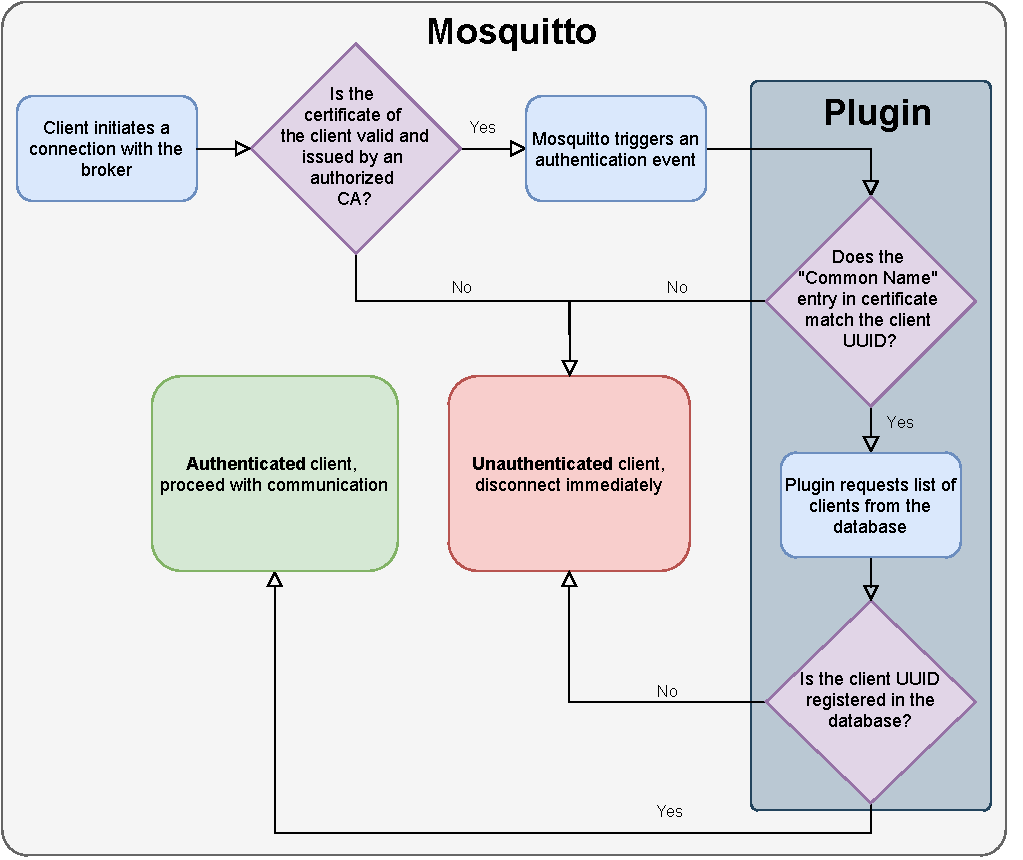
\includegraphics[width=0.7\linewidth]{images/mqtt authentication.pdf}
    \caption{Flowchart describing how a \acs{MQTT} client is authenticated by the \acs{MQTT} broker.}
    \label{fig:mqtt-plugin-authnflow}
\end{figure}

\paragraph{} Figure \ref{fig:mqtt-plugin-authzflow} describes how a client's request is authorized using this plugin. Since the client is already authenticated, Mosquitto proceeds by sending an authorization request for that client to the plugin. The plugin requests the list of permissions associated with the client role, and then checks if any permission on that list explicitly grants PUBLISH access to the topic.

\begin{figure}[H]
    \centering
    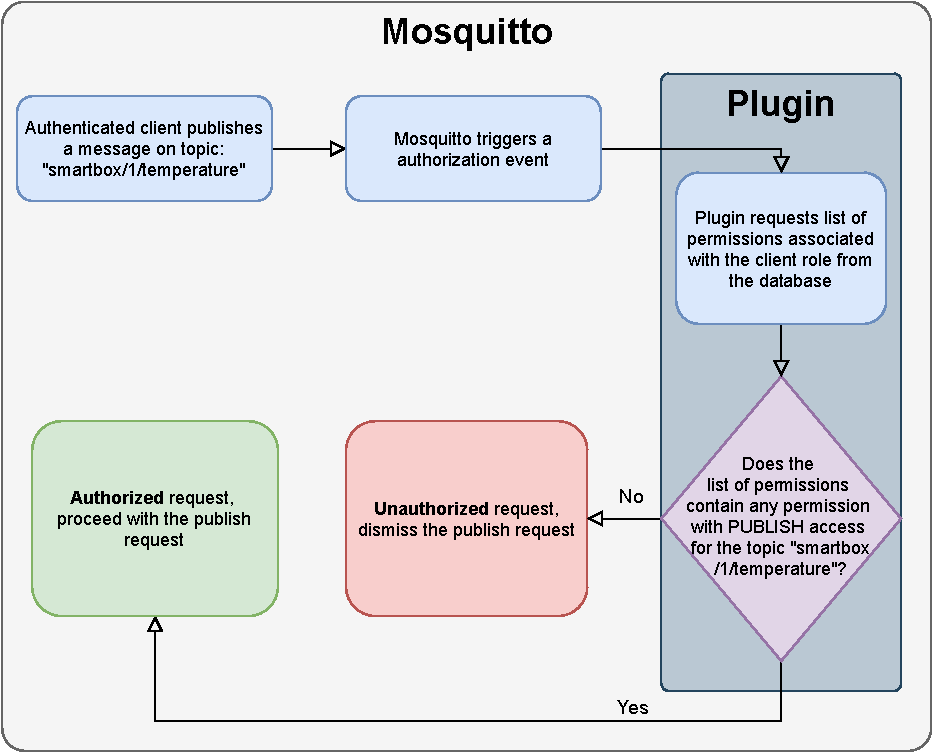
\includegraphics[width=0.7\linewidth]{images/mqtt authorization.pdf}
    \caption{Flowchart describing how an authenticated \acs{MQTT} client's request is authorized by the \acs{MQTT} broker.}
    \label{fig:mqtt-plugin-authzflow}
\end{figure}
\section{Data pre-processing}

The Data pre-processing service is used to process the incoming data from the \textit{Smart boxes} in real-time. It subscribes to incoming \acs{MQTT} messages using a \acs{MQTT} client with superuser privileges, that grants access to all topics. It validates the \acs{MQTT} messages according to the message formats specified in Section \ref{sec:mqtt payload format}, filters any irrelevant information, and stores it in the database. Currently, it does not apply any data analytics to detect critical conditions. The code for the service can be found here\footnote{\url{https://github.com/WoW-Institute-of-Systems-and-Robotics/gateway_pyservice}}. 

\paragraph{} Figure \ref{fig:dataprocess_flowdiagram} shows how incoming data is processed by the service. 

\begin{figure}[H]
    \centering
    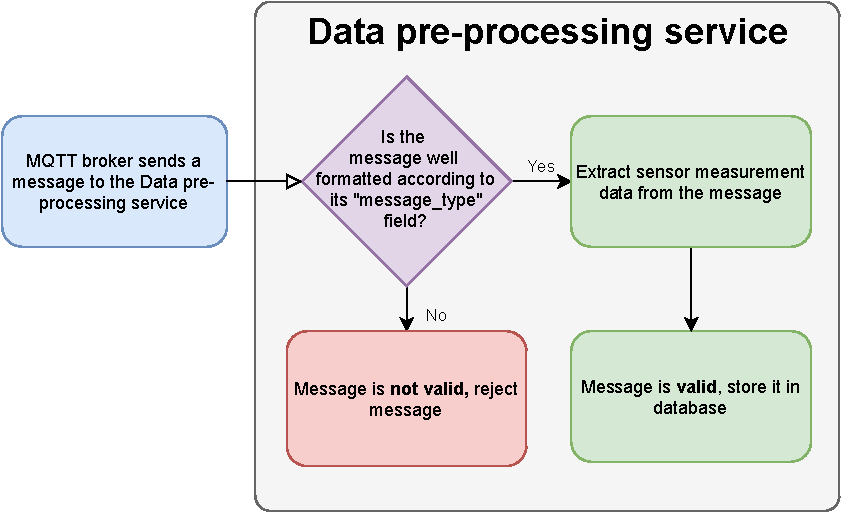
\includegraphics[width=0.7\linewidth]{images/data pre processing.pdf}
    \caption[Flowchart describing how incoming \acs{MQTT} messages are processed by the data pre-processing service.]{Flowchart describing how incoming \acs{MQTT} messages are processed by the data pre-processing service.}
    \label{fig:dataprocess_flowdiagram}
\end{figure}

\section{\acs{HIS} \acs{FHIR} Integration}
The \acs{HIS} \acs{FHIR} Integration service is used to manage the communication to and from GlobalCare \acs{HIS}. The service must implement a \acs{FHIR} \acs{HTTP} server \cite{fhir} capable of handling requests from the \acs{HIS}, as well as transform the sensor measurement data into \acs{FHIR} messages and communicate it to the \acs{HIS}.

\paragraph{} Out of the open-source implementations of the \acs{FHIR} specification available\footnote{\url{https://confluence.hl7.org/pages/viewpage.action?pageId=35718838}}, the HAPI FHIR Java library \cite{hapifhir} is one of the longest supported \acs{FHIR} implementations, with over 18 years of active development. The project is backed and maintained by Smile CDR\footnote{\url{https://www.smilecdr.com}}, a health technology company with a long-standing reputation in the health \acs{IT} field. The HAPI FHIR library also provides a simple and intuitive \acs{API} to interact with \acs{FHIR} resources \cite{fhir}, the objects used to represent any data in the protocol, handling all data parsing or serialization of data into \acs{FHIR} resources and vice versa.

\paragraph{} For these reasons HAPI FHIR Java library has been used to implement the \acs{FHIR} server. The software library provides several mechanisms to build \acs{FHIR} \acs{HTTP} servers. Although other models are available, the Plain Server model \cite{hapifhir} has been used to develop the \acs{FHIR} server since it just provides the bare-bones structure to build the \acs{API}, and not a full-fledged implementation with its own storage and functionality implemented, making it very flexible to work with. Using this model requires only  the implementation of how the \acs{FHIR} resource interactions translate to interactions with the data storage solution to create our own \acs{FHIR} server, while the HAPI FHIR handles all the \acs{HTTP} processing, as well as parsing and serialization of data into \acs{FHIR} resources. Even though \acs{FHIR} supports both \acf{XML} and \acf{JSON} data formats, only the \acs{JSON} data format is used for representing the \acs{FHIR} resources in the \acs{FHIR} server.

\paragraph{} The HAPI FHIR Plain Server implementation is based on Java Servlet 3.1 \acs{API}\footnote{\url{https://docs.oracle.com/javaee/7/tutorial/servlets.htm}}. Servlets are applications that are hosted on web servers, used to extend their capabilities. This means that in order to have a functional \acs{FHIR} server, a web server capable of hosting the HAPI FHIR Plain Server servlet is required. Since Eclipse Jetty9\footnote{\url{https://www.eclipse.org/jetty/}} is the web server used on the HAPI FHIR documentation, and is a relatively popular server (being used by Facebook, Google, Yahoo, etc.), it has been chosen for the development of the \acs{HIS} \acs{FHIR} Integration service. The code for the service can be found here\footnote{\url{https://github.com/WoW-Institute-of-Systems-and-Robotics/gateway_fhir_server/}}.

\paragraph{} In order to prepare the system for deployment in the first hospital trials, the development team has decided to use a pre-defined list of the subscriptions which remains static for the duration of the execution of the service. Additionally, the authentication protocol used on the \acs{FHIR} communication is Basic Authentication (using a static username and password), instead of the more secure option -- \textit{OAuth2} \footnote{\url{https://oauth.net/2/}} -- that was originally planned for implementation.

\subsection{FHIR Server} 

The servlet is composed by three major components:

\begin{itemize}
    \item ``Resource Providers'' -- defines the interactions with the \acs{FHIR} resources over \acs{HTTP} which are supported by our \acs{FHIR} server. It also invokes the \acs{CRUD} operations (create, read, update and delete) over our arbitrary data store through the ``Database Handler''.
    \item ``Database Handler'' -- defines how the \acs{FHIR} server connects to the data storage solution, which implements and exposes the methods used by the ``Resource Providers'' to interact with the data. This component is also responsible for translating the data as it is stored in the data storage solution into valid \acs{FHIR} resources and vice versa.
    \item ``Subscription Handler'' -- handles the scheduling and transmission of sensor data to the \acs{HIS} using \acs{FHIR} Observations \cite{fhir}.
\end{itemize}

\paragraph{} The Resource Providers define how and what resources are supported by the \acs{FHIR} server. Currently, the only interaction that is implemented is a \textit{read} operation \cite{fhir} on \acs{FHIR} Device resources \cite{fhir}. \acs{FHIR} Devices are the resources used to represent the \textit{Smart box} and \textit{Biosticker} sensors. Figure \ref{fig:fhir-get-device} shows how this interaction is processed by the \acs{FHIR} server.

\begin{figure}[H]
    \centering
    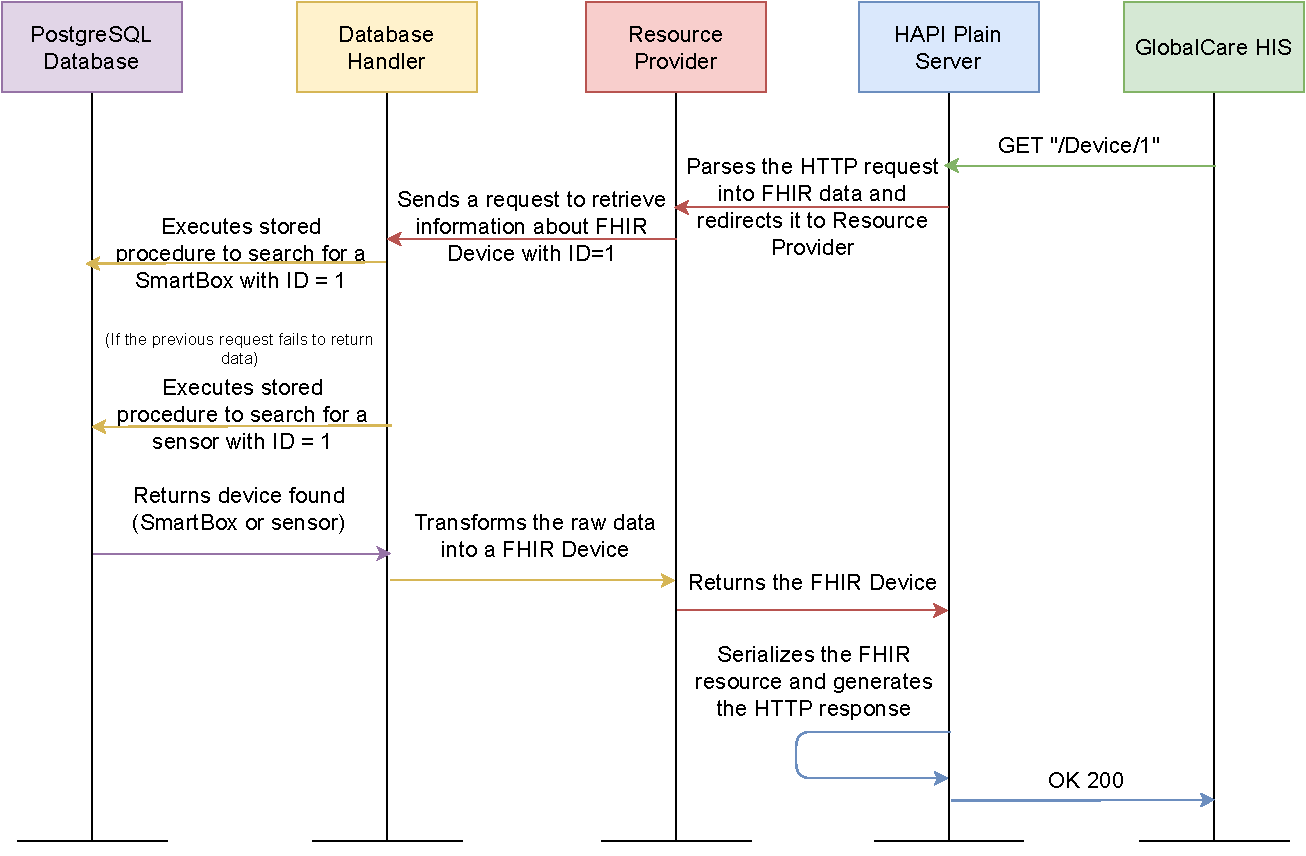
\includegraphics[width=\linewidth]{images/fhir get device.pdf}
    \caption[Sequence diagram describing the \textit{read} interaction on \acs{FHIR} Device resource.]{Sequence diagram describing the \textit{read} interaction on \acs{FHIR} Device resource. Although this is describing an interaction on the Device resources, the sequence diagram of a \textit{read} interaction on any other \acs{FHIR} resource should be very similar to this one.}
    \label{fig:fhir-get-device}
\end{figure} 

\paragraph{} As mentioned, the \acs{FHIR} Device resource is used to represent both the \textit{Smart box} and the \textit{Biosticker} sensors in the \acs{FHIR} protocol. To distinguish if a Device resource is a sensor or is a \textit{Smart box}, the resource uses the field ``Device.identifier'' to report the device's \acs{UUID}, and the field ``Device.type'' to describe the type of device using codes from an international health code-set\footnote{\url{https://www.snomed.org}}. Additionally, sensors are considered ``child'' Devices that must always have a parent Device associated to them. This means Device resources for sensors define the field ``Device.parent'', which must contain a reference to a \textit{Smart box}. The reader is referred to Appendix \ref{app:fhir_payloads} for the \acs{JSON} representation of the \acs{FHIR} resource for the \textit{Smart box} and for a sensor.

The reader is referred to Appendix \ref{app:fhir_payloads} for the \acs{JSON} representations of the \acs{FHIR} resources exchanged with the \acs{HIS}.

\paragraph{} The Subscription Handler is the component responsible for handling data subscription requests from the \acs{HIS}. To set up the subscriptions, after the \acs{FHIR} server initializes, the Subscription Handler sends a request to the Database Handler to retrieve the list of all active subscriptions. It then schedules tasks using the Quartz Scheduler library\footnote{\url{http://www.quartz-scheduler.org/}} according to the information specified in the subscription data, in order to trigger notification events periodically, as seen in Figure \ref{fig:fhir-post-bundle}. 

\paragraph{} The process is triggered by the Scheduler when there is a scheduled notification task at that given time. The \acs{FHIR} server parses the sensor data into its \acs{FHIR} representation, the \acs{FHIR} Observation resource, and then bundles it, using Bundle resource \cite{fhir}, with the \acs{FHIR} Device resources of the sensor and \textit{Smart box} associated to that sensor. This is necessary because the ``Interoperability'' layer on the GlobalCare \acs{HIS} does not hold information regarding the associations between the sensors and the \textit{Smart box}, and the associations with patients are performed in regard to the \textit{Smart box}, not the sensor. Instead, it relies on the \textit{Smart Gateway} to send that data, along with the measurement to properly process it. 

\clearpage

\begin{figure}[H]
    \centering
    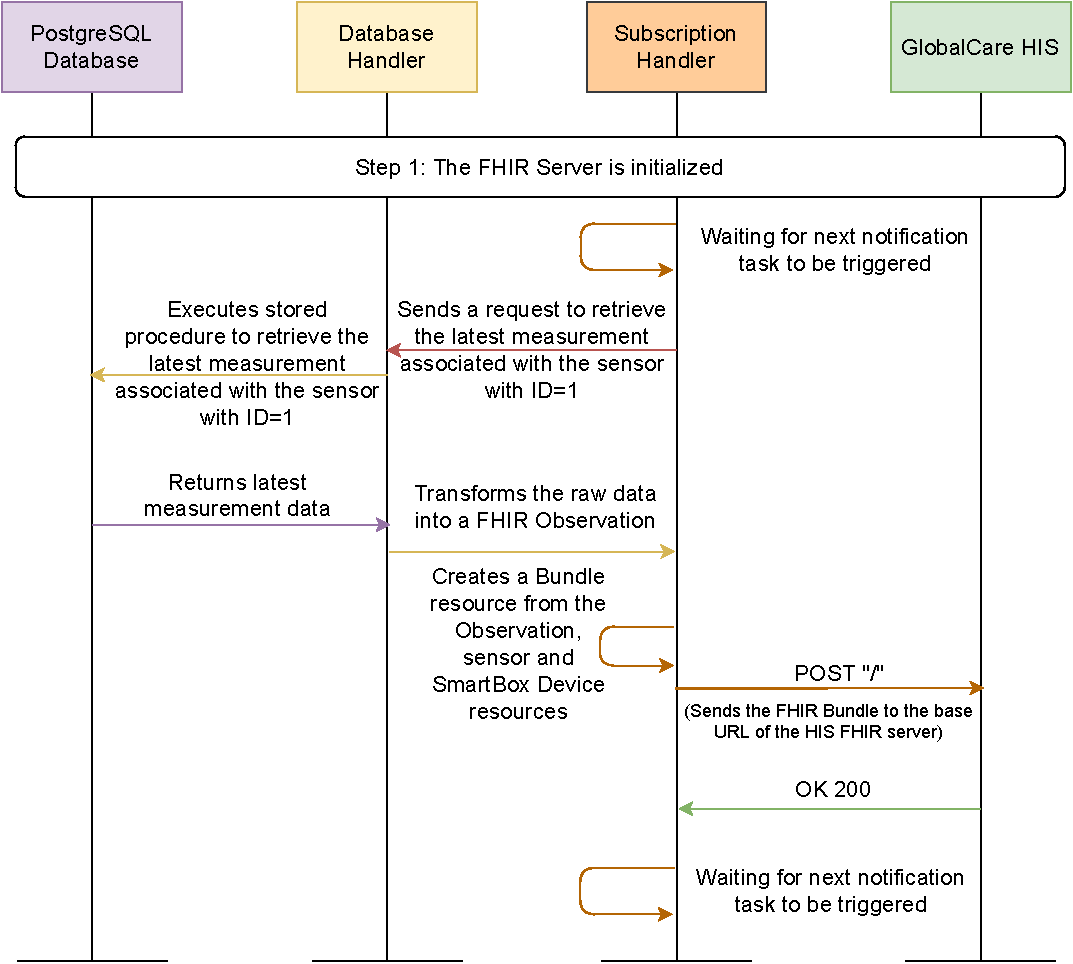
\includegraphics[width=\linewidth]{images/fhir post bundle.pdf}
    \caption[Sequence diagram describing the communication of sensor data to the \acs{HIS}.]{Sequence diagram describing the communication of sensor data to the \acs{HIS}.}
    \label{fig:fhir-post-bundle}
\end{figure} 

\section{Summary}

In this chapter, the different components which form the \textit{Smart Gateway} are presented. 
Next, the performance of the proposed solution is evaluated through a hospital trial and controlled lab tests.